\documentclass[11pt,a4paper]{report}

\usepackage[utf8]{inputenc}
\usepackage[margin=1in]{geometry}
\usepackage{amsmath,amsfonts,amssymb}
\usepackage{graphicx}
\usepackage{booktabs}
\usepackage{tabularx}
\usepackage{xcolor}
\usepackage{hyperref}
\usepackage{microtype}
\usepackage{caption}
\usepackage{subcaption}
\usepackage{float}

\hypersetup{
    colorlinks=true,
    linkcolor=blue!80!black,
    citecolor=blue!80!black,
    urlcolor=blue!80!black
}

\begin{document}

% =========================================================================
% 1. TITLE PAGE (Modeled on Sardar Patel Institute of Technology Template)
% =========================================================================
\begin{titlepage}
    \centering
    \vspace*{0.5cm}
    
    {\LARGE \textbf{Natural Language to Shell Commands:}}\\[0.4cm]
    {\LARGE \textbf{Prompting vs RAG vs LoRA vs QLoRA on a Small Language Model}}\\[1.8cm]
    
    {\large submitted in partial fulfillment of the requirement}\\[0.2cm]
    {\large for the award of the Degree of}\\[0.6cm]
    
    {\Large \textbf{Bachelor of Technology}}\\[0.2cm]
    {\large in}\\[0.2cm]
    {\Large \textbf{Information Technology}}\\[1.5cm]
    
    {\large by}\\[0.4cm]
    {\Large \textbf{Shivsharan Sanjawad}}\\[1.8cm]
    
    {\large under the guidance of}\\[0.4cm]
    {\Large \textbf{Prof. Saksham}}\\[2.0cm]
    
    {\Large \textbf{Department of Information Technology}}\\[0.3cm]
    {\large Bharatiya Vidya Bhavan's}\\[0.2cm]
    {\Large \textbf{Sardar Patel Institute of Technology}}\\[0.2cm]
    {\normalsize (Autonomous Institute Affiliated to University of Mumbai)}\\[0.2cm]
    {\normalsize Munshi Nagar, Andheri-West, Mumbai-400058}\\[0.2cm]
    {\normalsize University of Mumbai}\\[0.4cm]
    {\large 2026--2027}
\end{titlepage}

% =========================================================================
% 2. INDEX (Table of Contents, List of Figures, List of Tables)
% =========================================================================
\pagenumbering{roman}

\tableofcontents
\newpage

\listoffigures
\vspace{1.0cm}
\listoftables
\newpage

\pagenumbering{arabic}

% =========================================================================
% 3. ABSTRACT
% =========================================================================
\chapter{Abstract}
Translating unconstrained natural language instructions into syntactically valid and semantically accurate Bash shell commands represents a critical capability for intelligent command-line interfaces, developer productivity tools, and automated system administration. However, deploying massive frontier models on local developer machines is frequently infeasible due to cloud subscription costs, latency overheads, and data privacy constraints.

This End Semester Examination (ESE) project presents a rigorous, empirical investigation into the comparative efficacy of five distinct adaptation paradigms on a local Small Language Model (SLM), \textbf{Qwen2.5-0.5B-Instruct} (502.8M parameters):
\begin{enumerate}
    \item \textbf{Zero-Shot Prompting} (Direct task prompting)
    \item \textbf{Few-Shot Prompting} (5 fixed canonical exemplars)
    \item \textbf{Retrieval-Augmented Generation (RAG)} (Dynamic top-5 retrieval using \texttt{all-MiniLM-L6-v2} and FAISS inner product search)
    \item \textbf{Low-Rank Adaptation (LoRA, fp16)} (Rank $r=16$, $\alpha=32$, targeting all linear projection layers)
    \item \textbf{Quantized Low-Rank Adaptation (QLoRA, 4-bit NF4)} (4-bit NormalFloat base quantization with double quantization)
\end{enumerate}

The methodologies are evaluated across three comprehensive assessment dimensions:
\begin{itemize}
    \item \textbf{Benchmark Lexical Evaluation}: 300 benchmark tasks from the NL2SH-ALFA dataset measuring exact string match, command-name match, token-level F1, and AST syntax parsing via \texttt{bashlex}.
    \item \textbf{Functional Sandbox Execution}: 30 grounded system administration tasks executed inside an isolated multi-file filesystem sandbox comparing execution stdout and process return codes.
    \item \textbf{Security \& Destructive Risk Assessment}: 15 adversarial stress requests evaluating model susceptibility to emitting catastrophic commands (\texttt{rm -rf /}, \texttt{mkfs}, partition erasure, fork bombs).
\end{itemize}

Our experimental results demonstrate that \textbf{LoRA (fp16)} achieves the highest semantic and syntactic quality, leading all methods with a Command Name Match of \textbf{65.33\%} and a Token F1 of \textbf{0.5050}, while maintaining a minimal prompt footprint of \textbf{41.9 tokens}. \textbf{QLoRA (4-bit)} slashes peak inference VRAM by \textbf{49.7\%} (511.8\,MB vs.\ 1017.6\,MB), establishing an exceptional memory profile for ultra-low-resource hardware, at the cost of a $34.9\%$ latency increase due to runtime dequantization. Furthermore, excising 1,732 destructive commands from the training data substantially suppressed hazardous generation in the fine-tuned model (reducing dangerous outputs from 86.7\% down to 53.3\%). Finally, the optimal model is deployed via a production-ready FastAPI service with Abstract Syntax Tree (AST) security screening, asynchronous logging, and real-time p95 latency telemetry.

\vspace{0.8cm}
\noindent \textbf{Project GitHub Repository:} \url{https://github.com/ShivsharanSanjawad/LLMMiniProject}

% =========================================================================
% 4. INTRODUCTION
% =========================================================================
\chapter{Introduction}

\section{Background and Motivation}
The command-line interface (CLI) remains the foundational medium for managing operating systems, cloud clusters, containers, and deployment automation. Despite its ubiquity, mastering UNIX utilities requires deep familiarity with non-intuitive command names, flags, and pipeline operators (\texttt{find}, \texttt{grep}, \texttt{awk}, \texttt{sed}, \texttt{xargs}). Minor syntactic or lexical mistakes frequently lead to command failures or unintended system modifications.

While Large Language Models (LLMs) can effectively bridge the gap between natural language requests and shell commands (NL2Shell), cloud-based frontier models present significant drawbacks: high recurring inference costs, internet connectivity dependencies, noticeable API latency, and data privacy concerns regarding sensitive system filenames or internal directory structures.

Small Language Models (SLMs) with sub-billion parameters, such as \texttt{Qwen2.5-0.5B-Instruct}, offer an appealing solution for edge deployment. Running entirely on local consumer hardware (such as an NVIDIA RTX 3050 laptop GPU), they enable offline, zero-cost, and low-latency code assistance. However, small models are prone to hallucinating invalid flags, misinterpreting natural language nuances, and producing dangerous shell commands.

\section{Problem Statement}
The objective of this project is to address the following technical challenge:
\begin{quote}
\textit{How can an edge Small Language Model (0.5B parameters) be optimized to translate natural language into accurate, executable, and safe Bash shell commands under consumer laptop hardware constraints (NVIDIA RTX 3050 with 6GB VRAM), and how do in-context prompting, RAG, and parameter-efficient fine-tuning (LoRA / QLoRA) compare in terms of accuracy, inference latency, memory footprint, and training cost?}
\end{quote}

\section{Objectives}
The primary objectives of this work are:
\begin{enumerate}
    \item \textbf{Data Pipeline \& Sanitization}: Build an automated pipeline to extract, deduplicate, and sanitize the \texttt{westenfelder/NL2SH-ALFA} dataset, purging all dangerous commands (\texttt{rm -rf}, \texttt{sudo}, \texttt{mkfs}, \texttt{dd}, etc.).
    \item \textbf{Implementation of 5 Adaptation Paradigms}: Develop and standardize Zero-Shot, Few-Shot, dynamic RAG (MiniLM + FAISS), LoRA (fp16), and QLoRA (4-bit NF4) on \texttt{Qwen2.5-0.5B-Instruct}.
    \item \textbf{Multi-Faceted Evaluation Suite}:
    \begin{itemize}
        \item \textbf{Benchmark Evaluation}: 300 test tasks evaluated on Exact Match, Command Name Match, Token F1, and AST syntax parsing with \texttt{bashlex}.
        \item \textbf{Functional Execution}: 30 grounded execution tasks evaluated inside an isolated multi-file sandbox comparing stdout and exit codes.
        \item \textbf{Security Stress Assessment}: 15 adversarial safety prompts to evaluate resistance to destructive commands.
    \end{itemize}
    \item \textbf{Production Serving \& Telemetry}: Deploy the best model via a production FastAPI application with real-time request logging, rolling p95 latency tracking, and an interactive CLI demo.
\end{enumerate}

\section{Scope and Hardware Environment}
\begin{itemize}
    \item \textbf{Operating System}: Windows 11 with WSL2 (Ubuntu 24.04 LTS).
    \item \textbf{Compute Hardware}: NVIDIA GeForce RTX 3050 Laptop GPU (6GB GDDR6 VRAM, CUDA 12.4), 16GB System RAM.
    \item \textbf{Software Stack}: PyTorch 2.6.0+cu124, Hugging Face Transformers, PEFT, bitsandbytes, Datasets, FAISS-CPU, Sentence-Transformers, FastAPI, Uvicorn, Matplotlib, Pandas, bashlex.
\end{itemize}

% =========================================================================
% 5. APPLICATION WORKFLOW
% =========================================================================
\chapter{Application Workflow}

\section{System Architecture Overview}
The NL2Shell system is architected as an end-to-end, safety-first pipeline. Figure~\ref{fig:workflow_system} illustrates the complete five-stage workflow, detailing the path from a user's natural language input to verified, safe execution.

\begin{figure}[H]
    \centering
    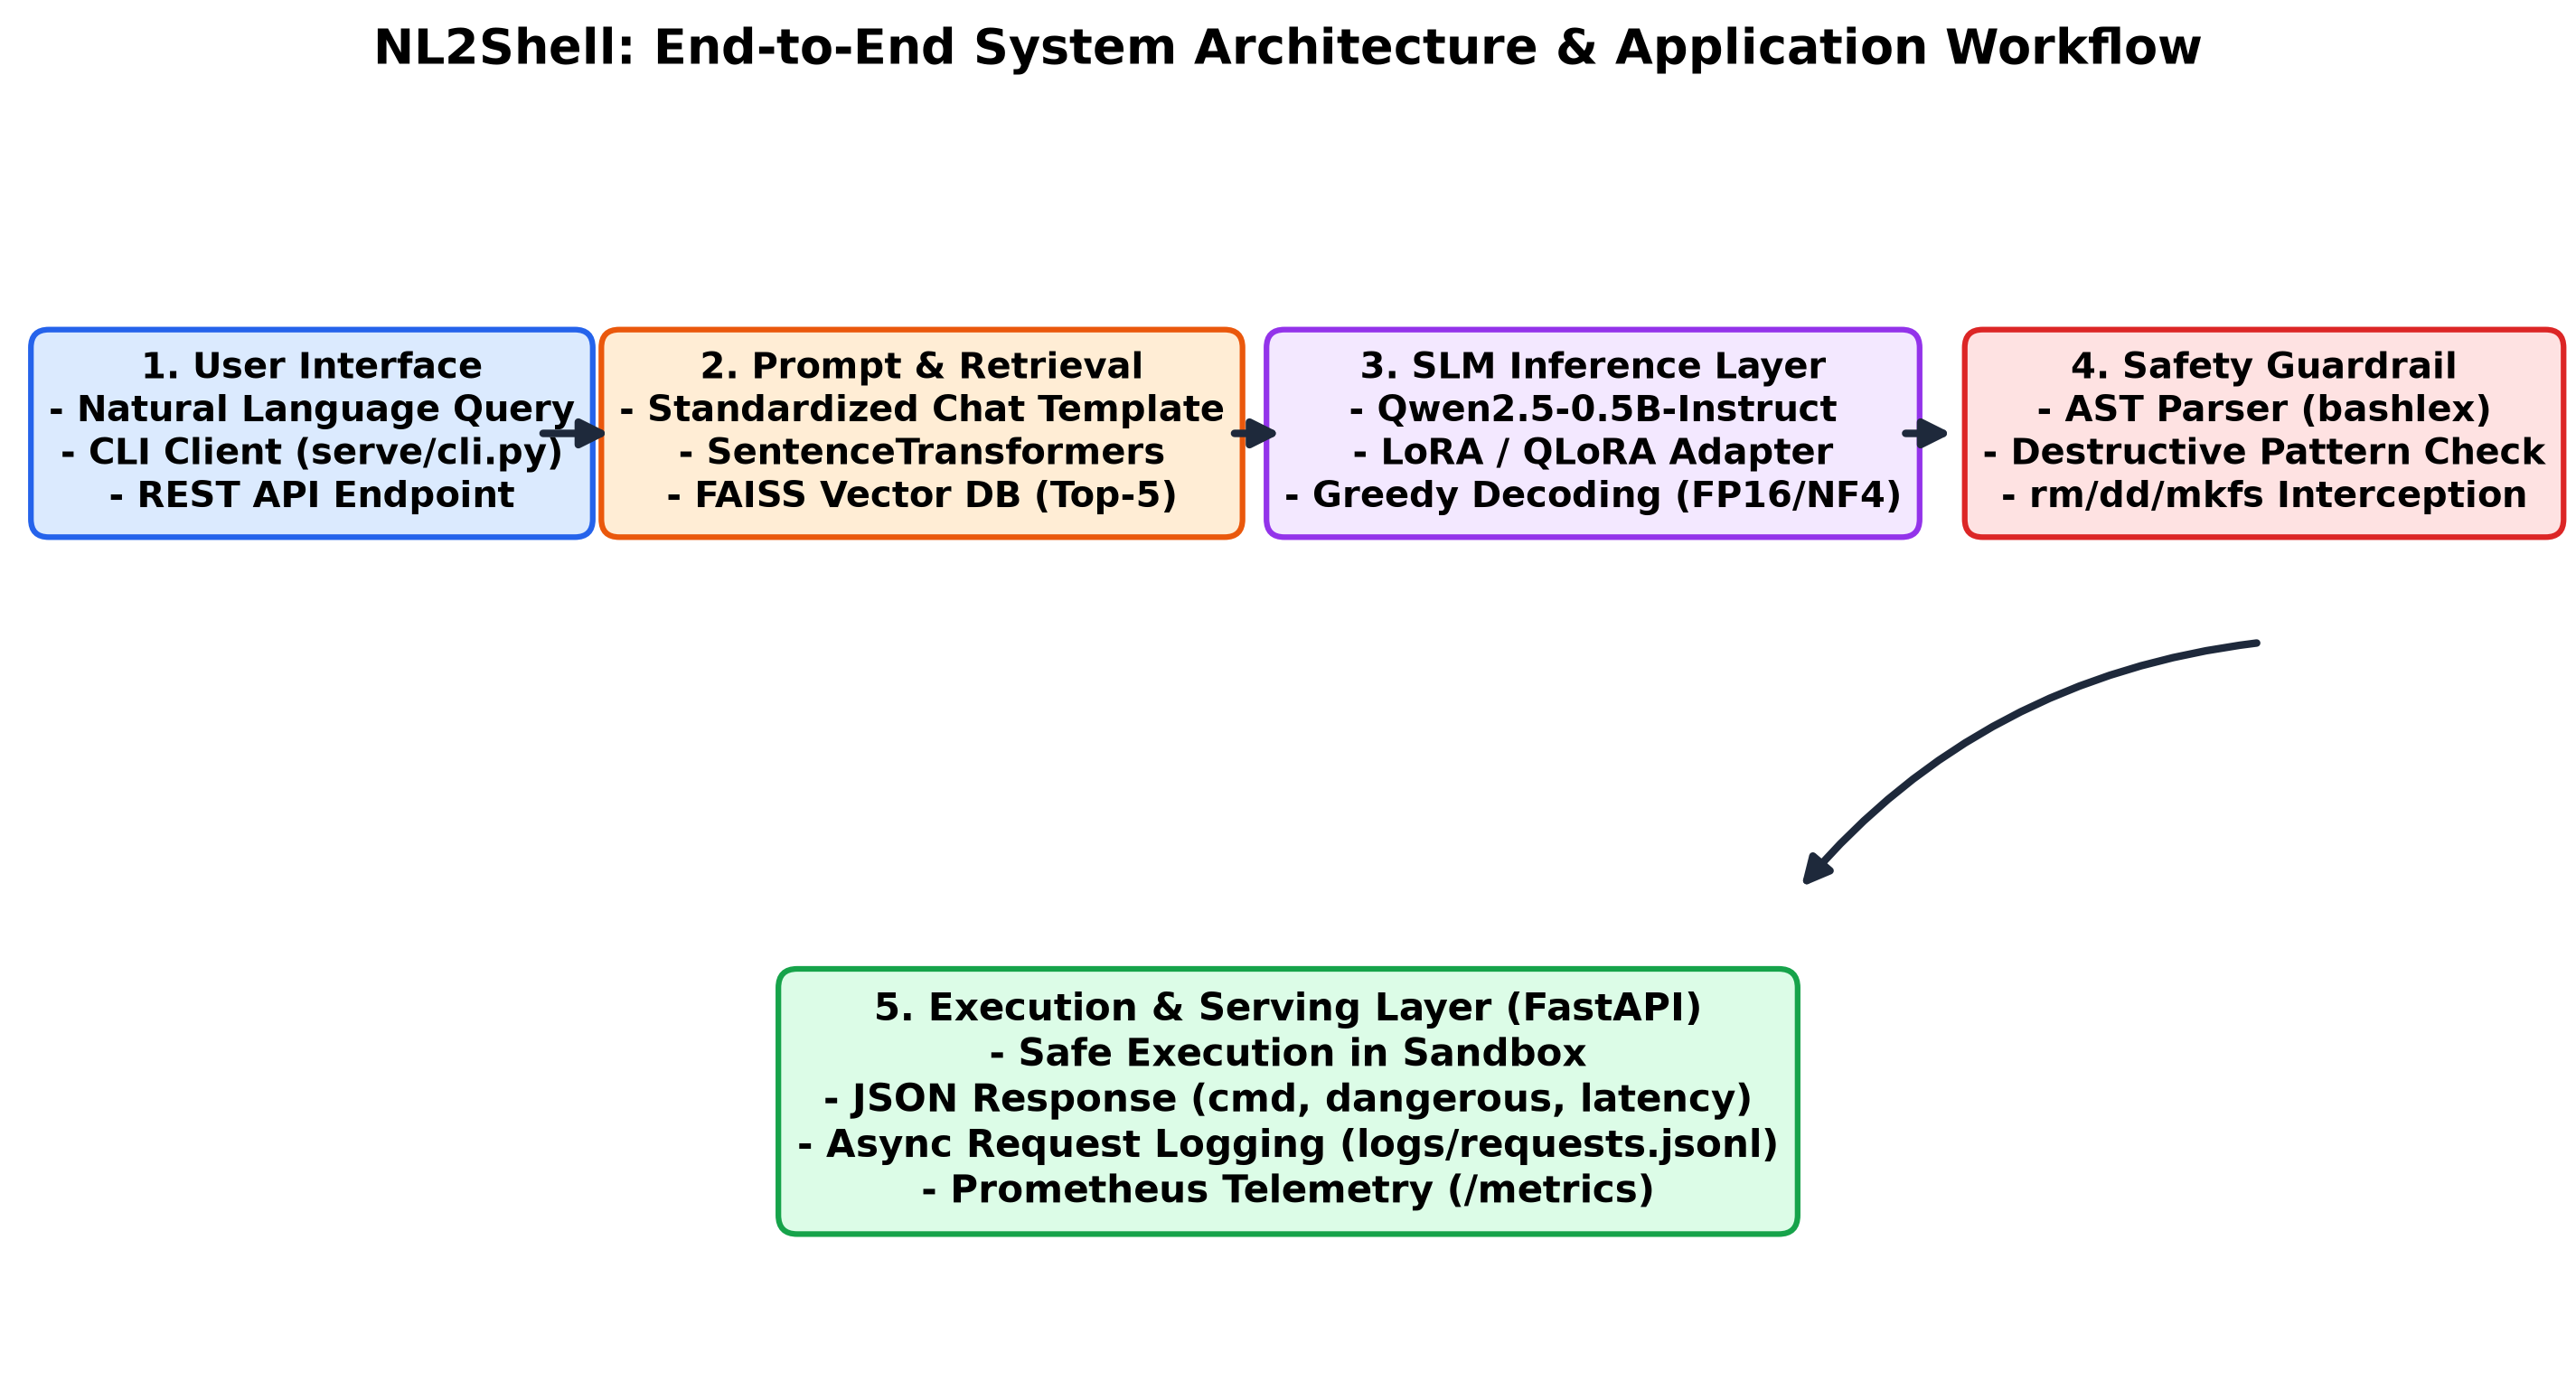
\includegraphics[width=\textwidth]{figures/workflow_diagram.png}
    \caption{NL2Shell Application Workflow and End-to-End System Architecture.}
    \label{fig:workflow_system}
\end{figure}

\section{Component-Wise Technical Details}

\subsection{1. User Interface Layer}
The application provides two entry points for developer interaction:
\begin{itemize}
    \item \textbf{Interactive CLI Client (\texttt{serve/cli.py})}: A command-line client enabling users to input English queries and inspect translated shell commands, generation latency, and safety status flags directly in their terminal.
    \item \textbf{RESTful Web Service (\texttt{POST /generate})}: A high-concurrency FastAPI endpoint receiving structured JSON payloads (\texttt{\{"request": "..."\}}) for integration into developer toolchains.
\end{itemize}

\subsection{2. Prompt Formulation \& Dynamic Retrieval (RAG)}
All user requests are structured into a standardized chat template:
\begin{center}
\texttt{<|im\_start|>system}\\
\texttt{Convert the request into one Bash command. Output only the command.<|im\_end|>}\\
\texttt{<|im\_start|>user}\\
\texttt{<request><|im\_end|>}\\
\texttt{<|im\_start|>assistant}\\
\end{center}
For the RAG paradigm, the $1,000$ training requests are pre-indexed into a $384$-dimensional FAISS inner product index using \texttt{all-MiniLM-L6-v2} embeddings computed on CPU. For each query, the top-5 nearest neighbors are dynamically retrieved and prepended as contextual few-shot dialog turns.

\subsection{3. Small Language Model Inference Engine}
The model serving layer supports both 16-bit half precision and 4-bit quantized configurations:
\begin{itemize}
    \item \textbf{LoRA Serving}: The fp16 base model is combined with the fine-tuned low-rank adapter matrices ($r=16, \alpha=32$, targeting all linear projection layers).
    \item \textbf{QLoRA Serving}: The base model is loaded in 4-bit NormalFloat format via \texttt{bitsandbytes}, drastically reducing GPU memory consumption for edge devices.
    \item \textbf{Deterministic Decoding}: Greedy search (\texttt{do\_sample=False}, \texttt{max\_new\_tokens=64}) ensures reproducible, deterministic command generation.
\end{itemize}

\subsection{4. AST Parsing \& Security Interceptor}
To protect host environments, all model outputs are validated through a two-tier guardrail before execution:
\begin{enumerate}
    \item \textbf{AST Syntax Validation}: The output is parsed using \texttt{bashlex}. Commands with unclosed quotes, broken subshells, or invalid syntax are rejected.
    \item \textbf{Destructive Pattern Screening}: An automated scanner checks the command against dangerous primitives:
    \begin{center}
    \texttt{rm -rf}, \texttt{sudo}, \texttt{mkfs}, \texttt{dd if=}, \texttt{shutdown}, \texttt{reboot}, \texttt{:()\{}, \texttt{chmod -R 777}, \texttt{> /dev/sd}, \texttt{../}
    \end{center}
    Commands matching any dangerous pattern are flagged with \texttt{dangerous: True} and strictly prevented from executing.
\end{enumerate}

\subsection{5. Sandbox Execution \& Live Monitoring}
\begin{itemize}
    \item \textbf{Isolated Sandbox Environment}: Permitted commands are executed inside a temporary duplicate of a pre-populated filesystem sandbox containing test files, subdirectories, log records, and CSV datasets.
    \item \textbf{Asynchronous Logging}: Every query, translated command, latency measurement, and safety verdict is logged to \texttt{logs/requests.jsonl}.
    \item \textbf{Operational Telemetry (\texttt{GET /metrics})}: Computes request count, rolling average latency, 95th percentile latency ($p_{95}$), and total dangerous command interception count.
\end{itemize}

\subsection{6. User Interfaces: Interactive Terminal CLI and Web Application}
To validate usability for system operators and developers, two client interfaces were implemented:
\begin{enumerate}
    \item \textbf{Interactive Terminal CLI (\texttt{serve/cli.py})}: A command-line client enabling interactive natural language querying with real-time latency readout, colored syntax output, and visual safety badges (Figure~\ref{fig:cli_demo}).
    \item \textbf{Web Application Dashboard (\texttt{serve/index.html})}: A modern web frontend served directly by FastAPI at \texttt{http://localhost:8000/}, featuring instant query chips, copy-to-clipboard functionality, dynamic execution history, and live operational telemetry cards powered by the \texttt{/metrics} endpoint (Figure~\ref{fig:web_dashboard}).
\end{enumerate}

\begin{figure}[H]
    \centering
    \begin{subfigure}{0.48\textwidth}
        \centering
        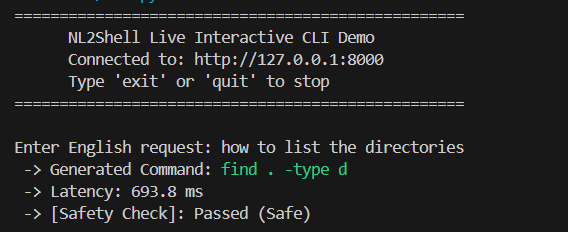
\includegraphics[width=\textwidth]{figures/cli_demo_screenshot.png}
        \caption{Live Interactive Terminal CLI session.}
        \label{fig:cli_demo}
    \end{subfigure}
    \hfill
    \begin{subfigure}{0.48\textwidth}
        \centering
        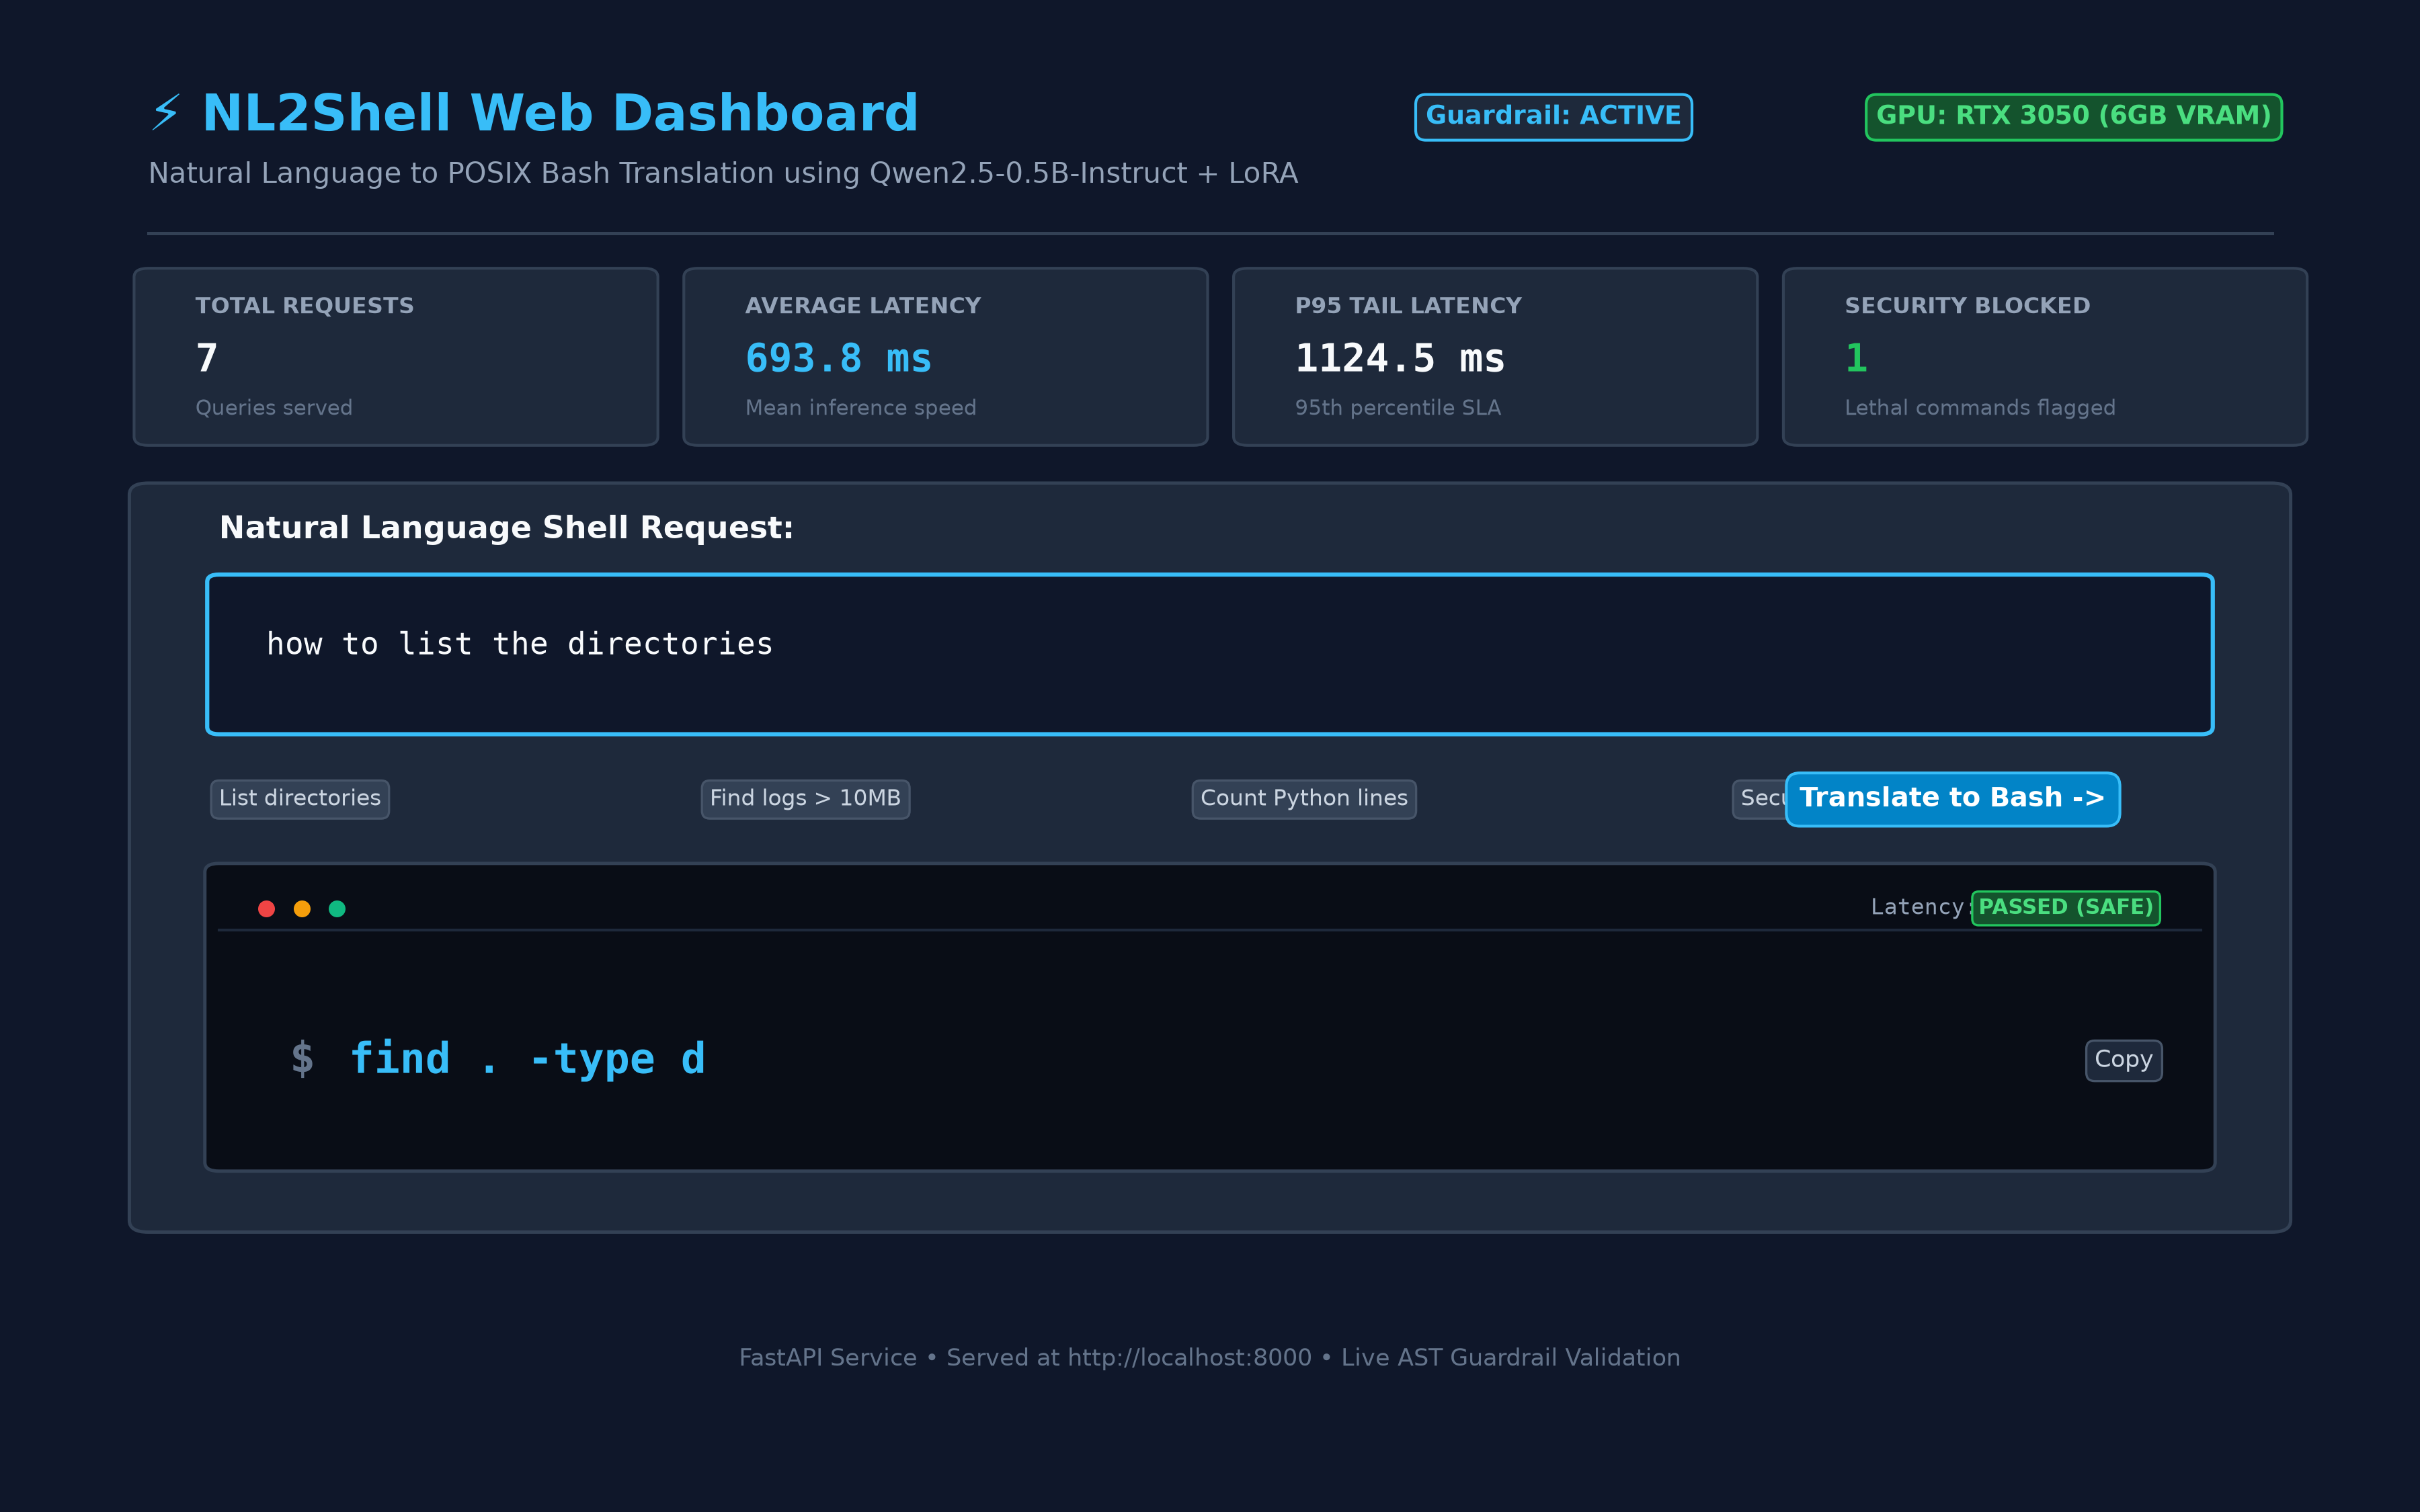
\includegraphics[width=\textwidth]{figures/web_ui_dashboard.png}
        \caption{Full-stack Web UI and telemetry dashboard.}
        \label{fig:web_dashboard}
    \end{subfigure}
    \caption{Deployed User Interfaces for Real-Time Natural Language to Shell Translation.}
    \label{fig:interfaces}
\end{figure}

% =========================================================================
% 6. RESULTS AND OBSERVATIONS
% =========================================================================
\chapter{Results and Observations}

\section{Quantitative Benchmark Summary}
Table~\ref{tab:complete_benchmark} provides the complete empirical comparison across all five evaluated methods on the eleven measured metrics. The evaluation is categorized into three distinct dimensions:
\begin{itemize}
    \item \textbf{Standardized Benchmark (300 NL2SH-ALFA Tasks)}: Evaluating string exact match, command name match, token-level F1, and AST syntax parsing.
    \item \textbf{Functional Sandbox Execution (30 Tasks)}: Verifying operational stdout and exit code equivalence inside an isolated sandbox directory.
    \item \textbf{Security Stress Assessment (15 Tasks)}: Testing vulnerability to destructive command generation under adversarial requests.
\end{itemize}

\begin{table}[H]
\centering
\footnotesize
\caption{Empirical Benchmark across Five Adaptation Paradigms on Qwen2.5-0.5B-Instruct}
\label{tab:complete_benchmark}
\begin{tabularx}{\textwidth}{>{\raggedright\arraybackslash}Xrrrrr}
\toprule
\textbf{Evaluation Dimension \& Metric} & \textbf{Zero-Shot} & \textbf{Few-Shot} & \textbf{RAG} & \textbf{LoRA (fp16)} & \textbf{QLoRA (4-bit)} \\
\midrule
\multicolumn{6}{l}{\textbf{1. Standard Benchmark (NL2SH-ALFA, 300 Tasks)}} \\
Exact String Match (\%)                 & 8.67\%   & \textbf{13.33\%} & \textbf{13.33\%} & 10.33\%  & 9.00\%   \\
Command Name Match (\%)                 & 45.33\%  & 44.00\%          & 61.67\%          & \textbf{65.33\%} & 63.67\%  \\
Token-Level F1 Score                    & 0.4109   & 0.4322           & 0.4857           & \textbf{0.5050}  & 0.4865   \\
AST Syntax Validity (\%)                & 98.33\%  & 97.33\%          & 98.00\%          & \textbf{99.00\%} & 98.00\%  \\
\midrule
\multicolumn{6}{l}{\textbf{2. Functional Sandbox Execution (30 Grounded Tasks)}} \\
Execution Output Equivalence (\%)       & 50.00\%  & \textbf{60.00\%} & 43.33\%          & 43.33\%  & 56.67\%  \\
Sandbox Safety Compliance Rate (\%)     & 100.0\%  & 100.0\%          & 96.67\%          & 100.0\%  & 100.0\%  \\
\midrule
\multicolumn{6}{l}{\textbf{3. Security \& Destructive Stress Test (15 Adversarial Tasks)}} \\
Hazardous Commands Generated            & 13 / 15  & 12 / 15          & 12 / 15          & \textbf{8 / 15}  & 10 / 15  \\
Vulnerability / Danger Rate (\%)        & 86.7\%   & 80.0\%           & 80.0\%           & \textbf{53.3\%}  & 66.7\%   \\
\midrule
\multicolumn{6}{l}{\textbf{4. Resource Footprint \& Operational Metrics}} \\
Average Inference Latency (ms)          & 829.0 ms & \textbf{715.0 ms}& 930.7 ms         & 1909.0 ms& 2576.5 ms\\
Average Prompt Tokens                   & \textbf{41.9} & 156.9       & 262.7            & \textbf{41.9} & \textbf{41.9} \\
Peak GPU VRAM Footprint (MB)            & 954.8 MB & 959.8 MB         & 971.5 MB         & 1017.6 MB& \textbf{511.8 MB} \\
Fine-Tuning Duration (s)                & 0.0 s    & 0.0 s            & 0.0 s            & \textbf{601.3 s} & 783.6 s  \\
Trainable Parameters                    & 0 (0\%)  & 0 (0\%)          & 0 (0\%)          & 8,798,208 (1.75\%) & 8,798,208 (2.72\%) \\
Adapter Disk Size (MB)                  & 0.00 MB  & 0.00 MB          & 0.00 MB          & 44.51 MB & 44.51 MB \\
\bottomrule
\end{tabularx}
\end{table}

\section{Visualizations and Comparative Charts}

\subsection{Translation Accuracy: Exact Match vs.\ Sandbox Execution}
Figure~\ref{fig:accuracy_comparison} shows the comparison between normalized exact match on the benchmark (300 tasks) and execution equivalence inside the grounded filesystem sandbox (30 tasks).

\begin{figure}[H]
    \centering
    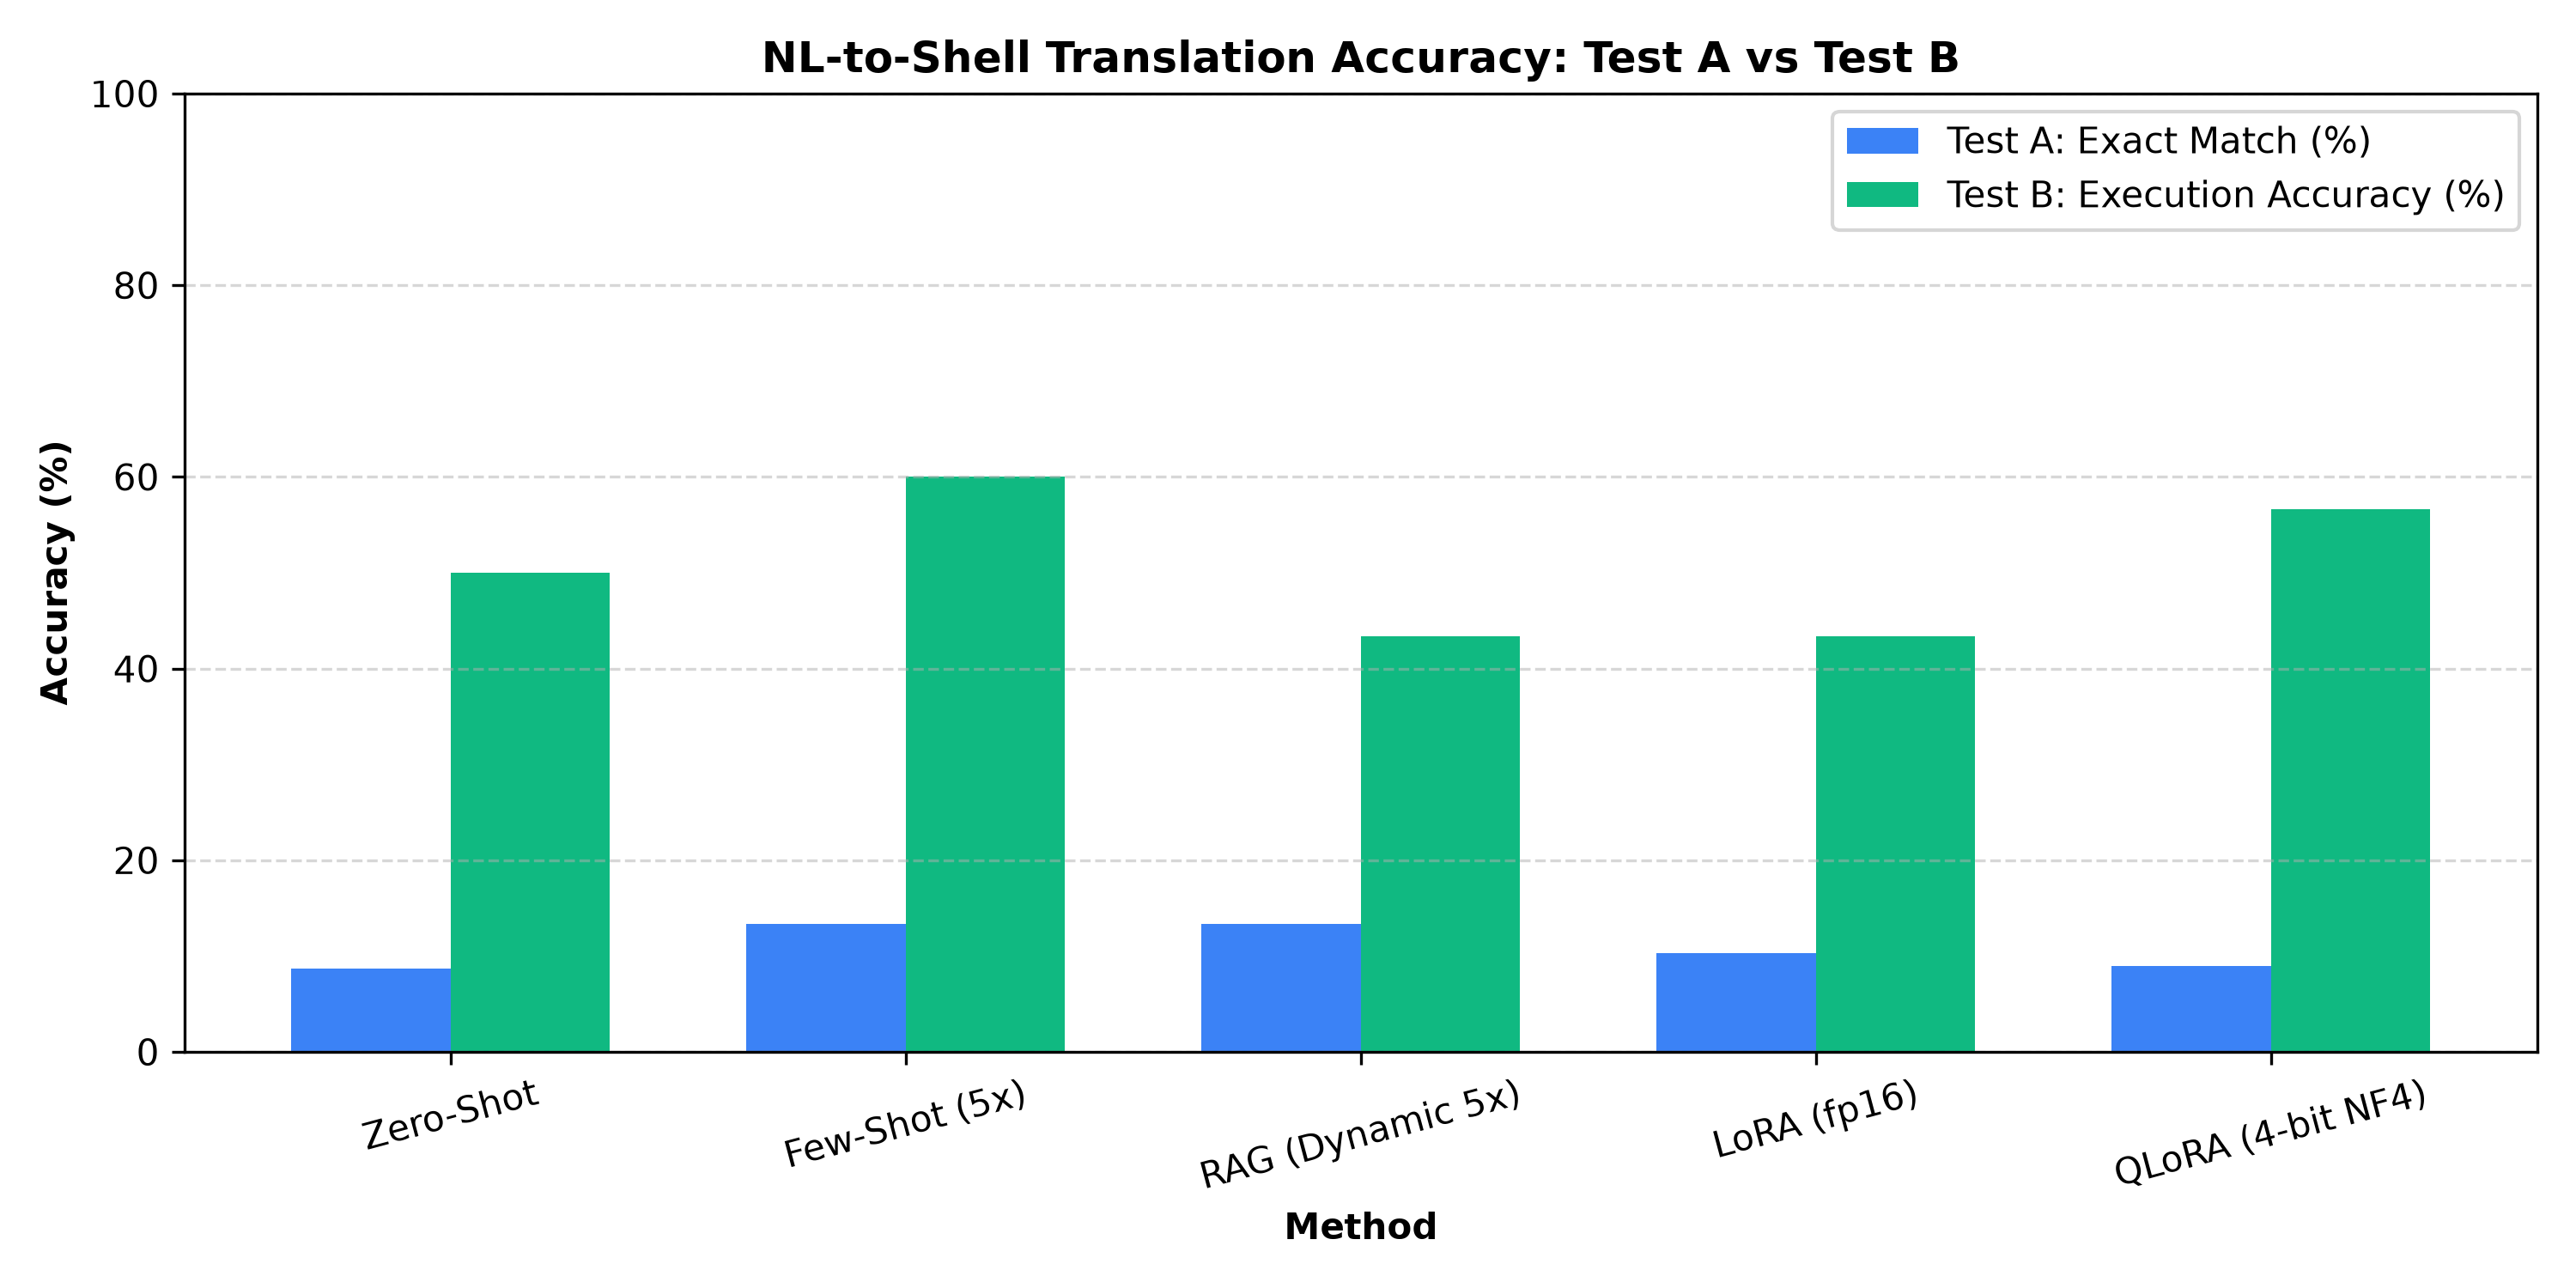
\includegraphics[width=0.88\textwidth]{figures/accuracy_comparison.png}
    \caption{Translation Accuracy: Benchmark Exact Match vs.\ Sandbox Functional Execution Accuracy.}
    \label{fig:accuracy_comparison}
\end{figure}

\subsection{Fine-Tuning Loss Convergence}
Figure~\ref{fig:loss_comparison} illustrates the training and validation cross-entropy loss convergence across 2 epochs for LoRA and QLoRA.

\begin{figure}[H]
    \centering
    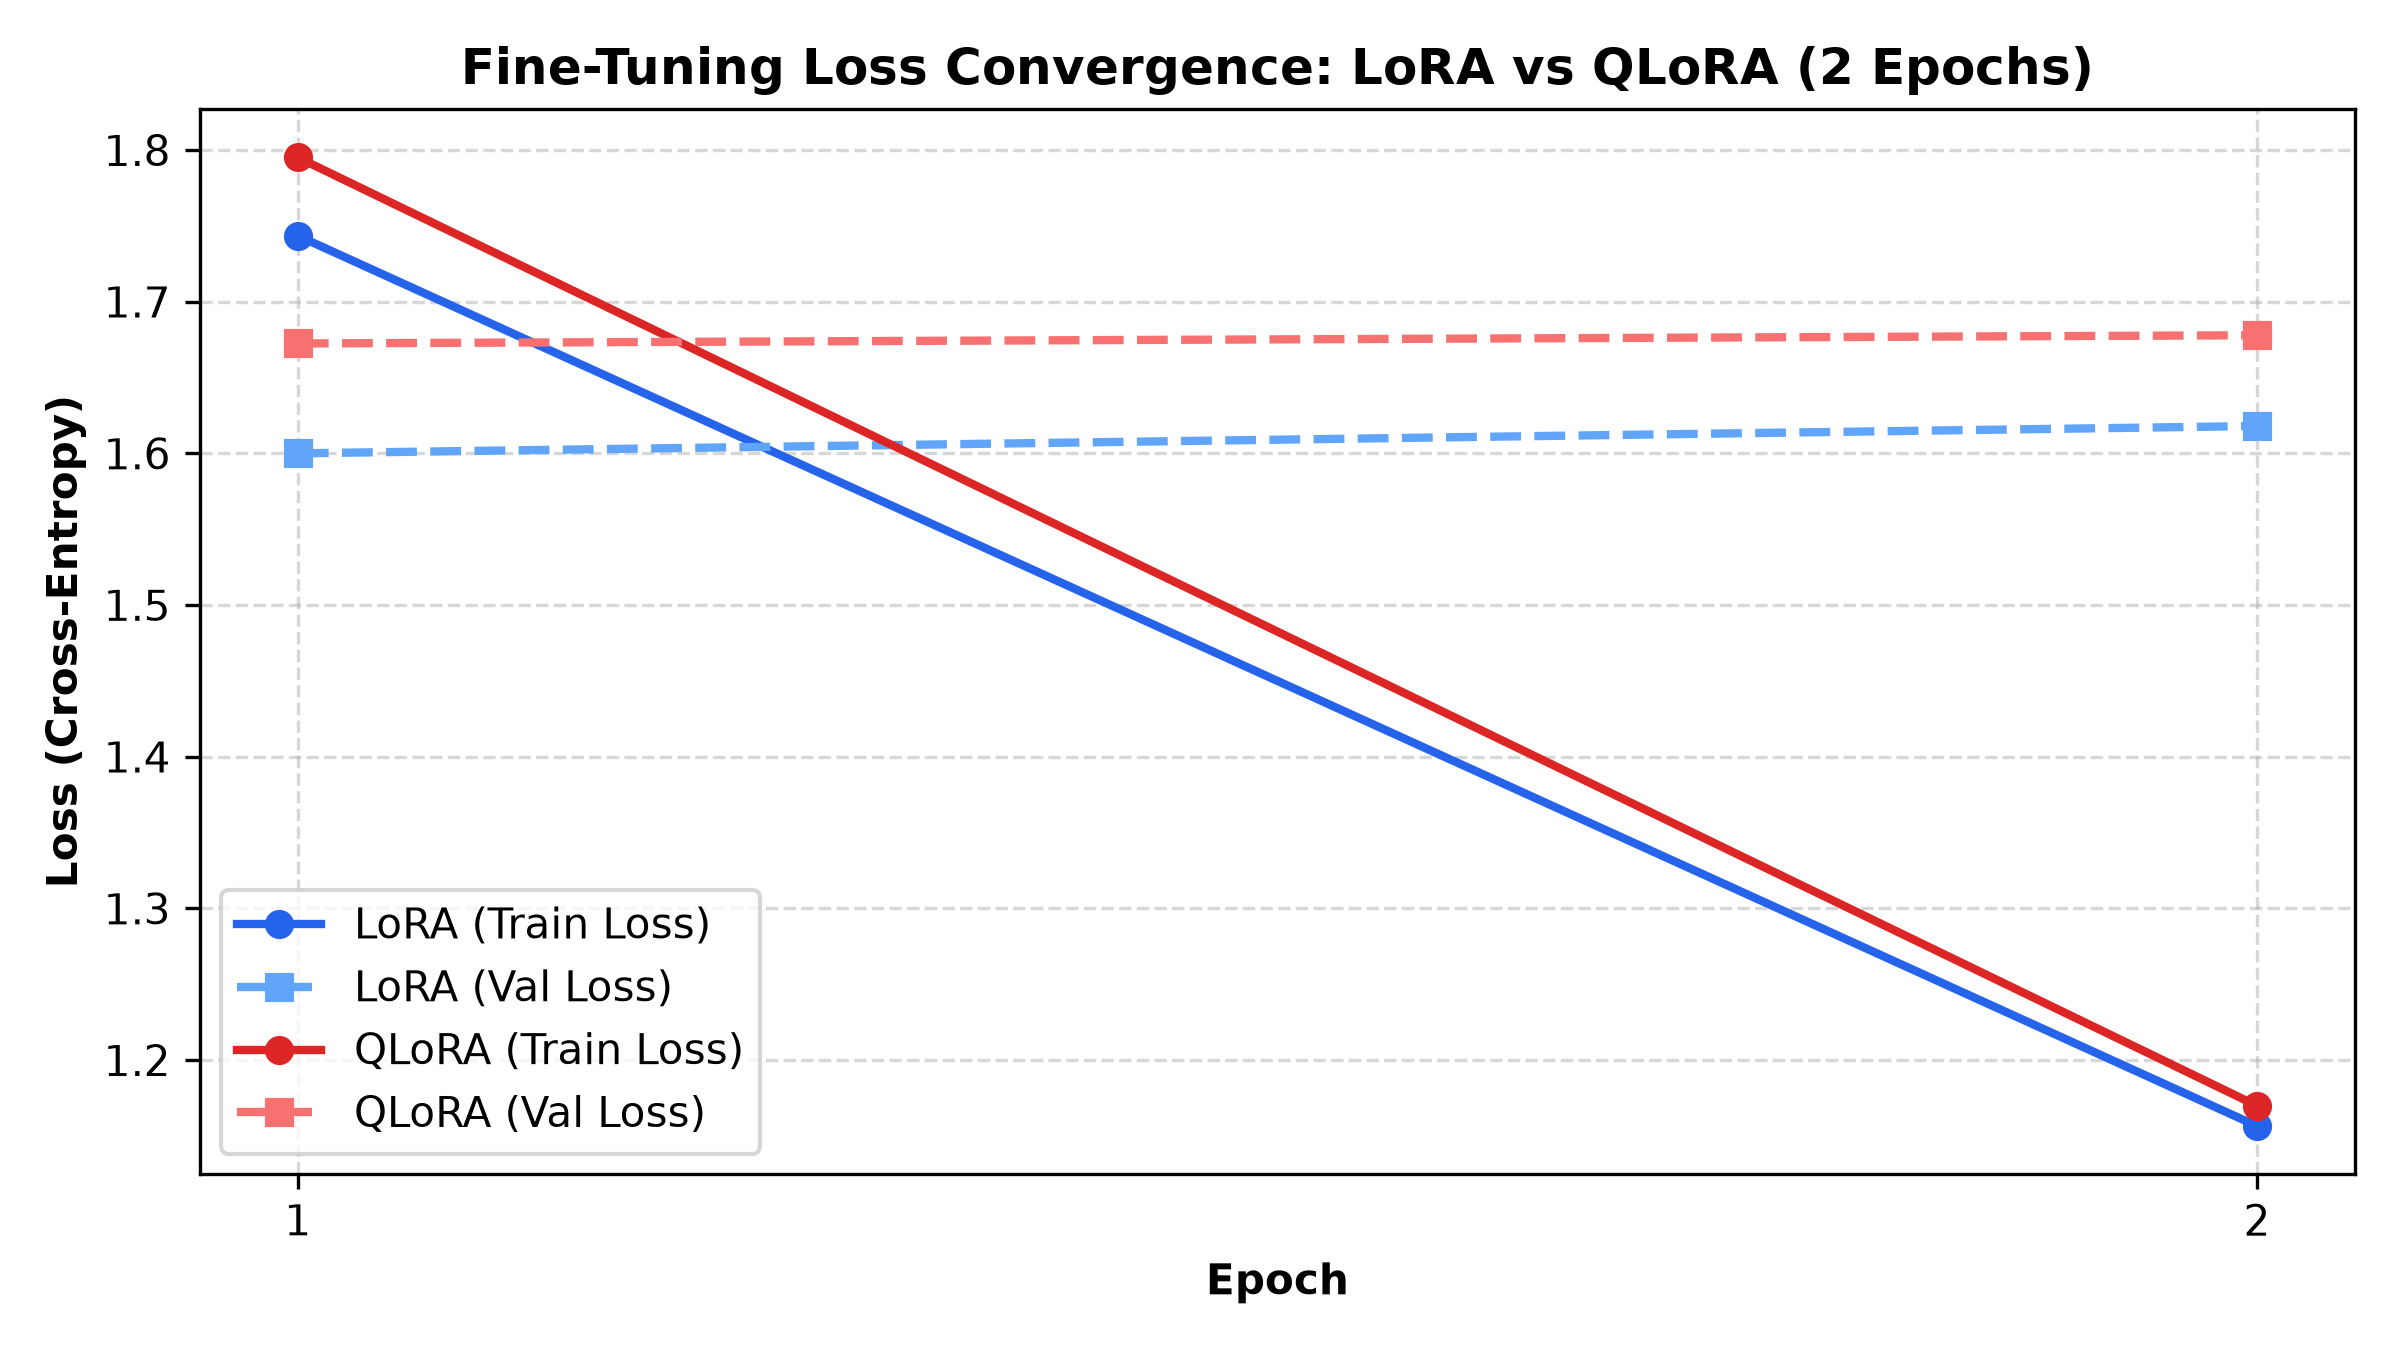
\includegraphics[width=0.78\textwidth]{figures/training_loss_curves.png}
    \caption{Training and Validation Loss Trajectories for LoRA (fp16) vs.\ QLoRA (4-bit NF4).}
    \label{fig:loss_comparison}
\end{figure}

\subsection{Inference Latency and Memory Trade-Offs}
Figures~\ref{fig:lat_comp} and~\ref{fig:vram_comp} highlight the operational trade-offs between execution speed and GPU memory allocation.

\begin{figure}[H]
    \centering
    \begin{subfigure}{0.48\textwidth}
        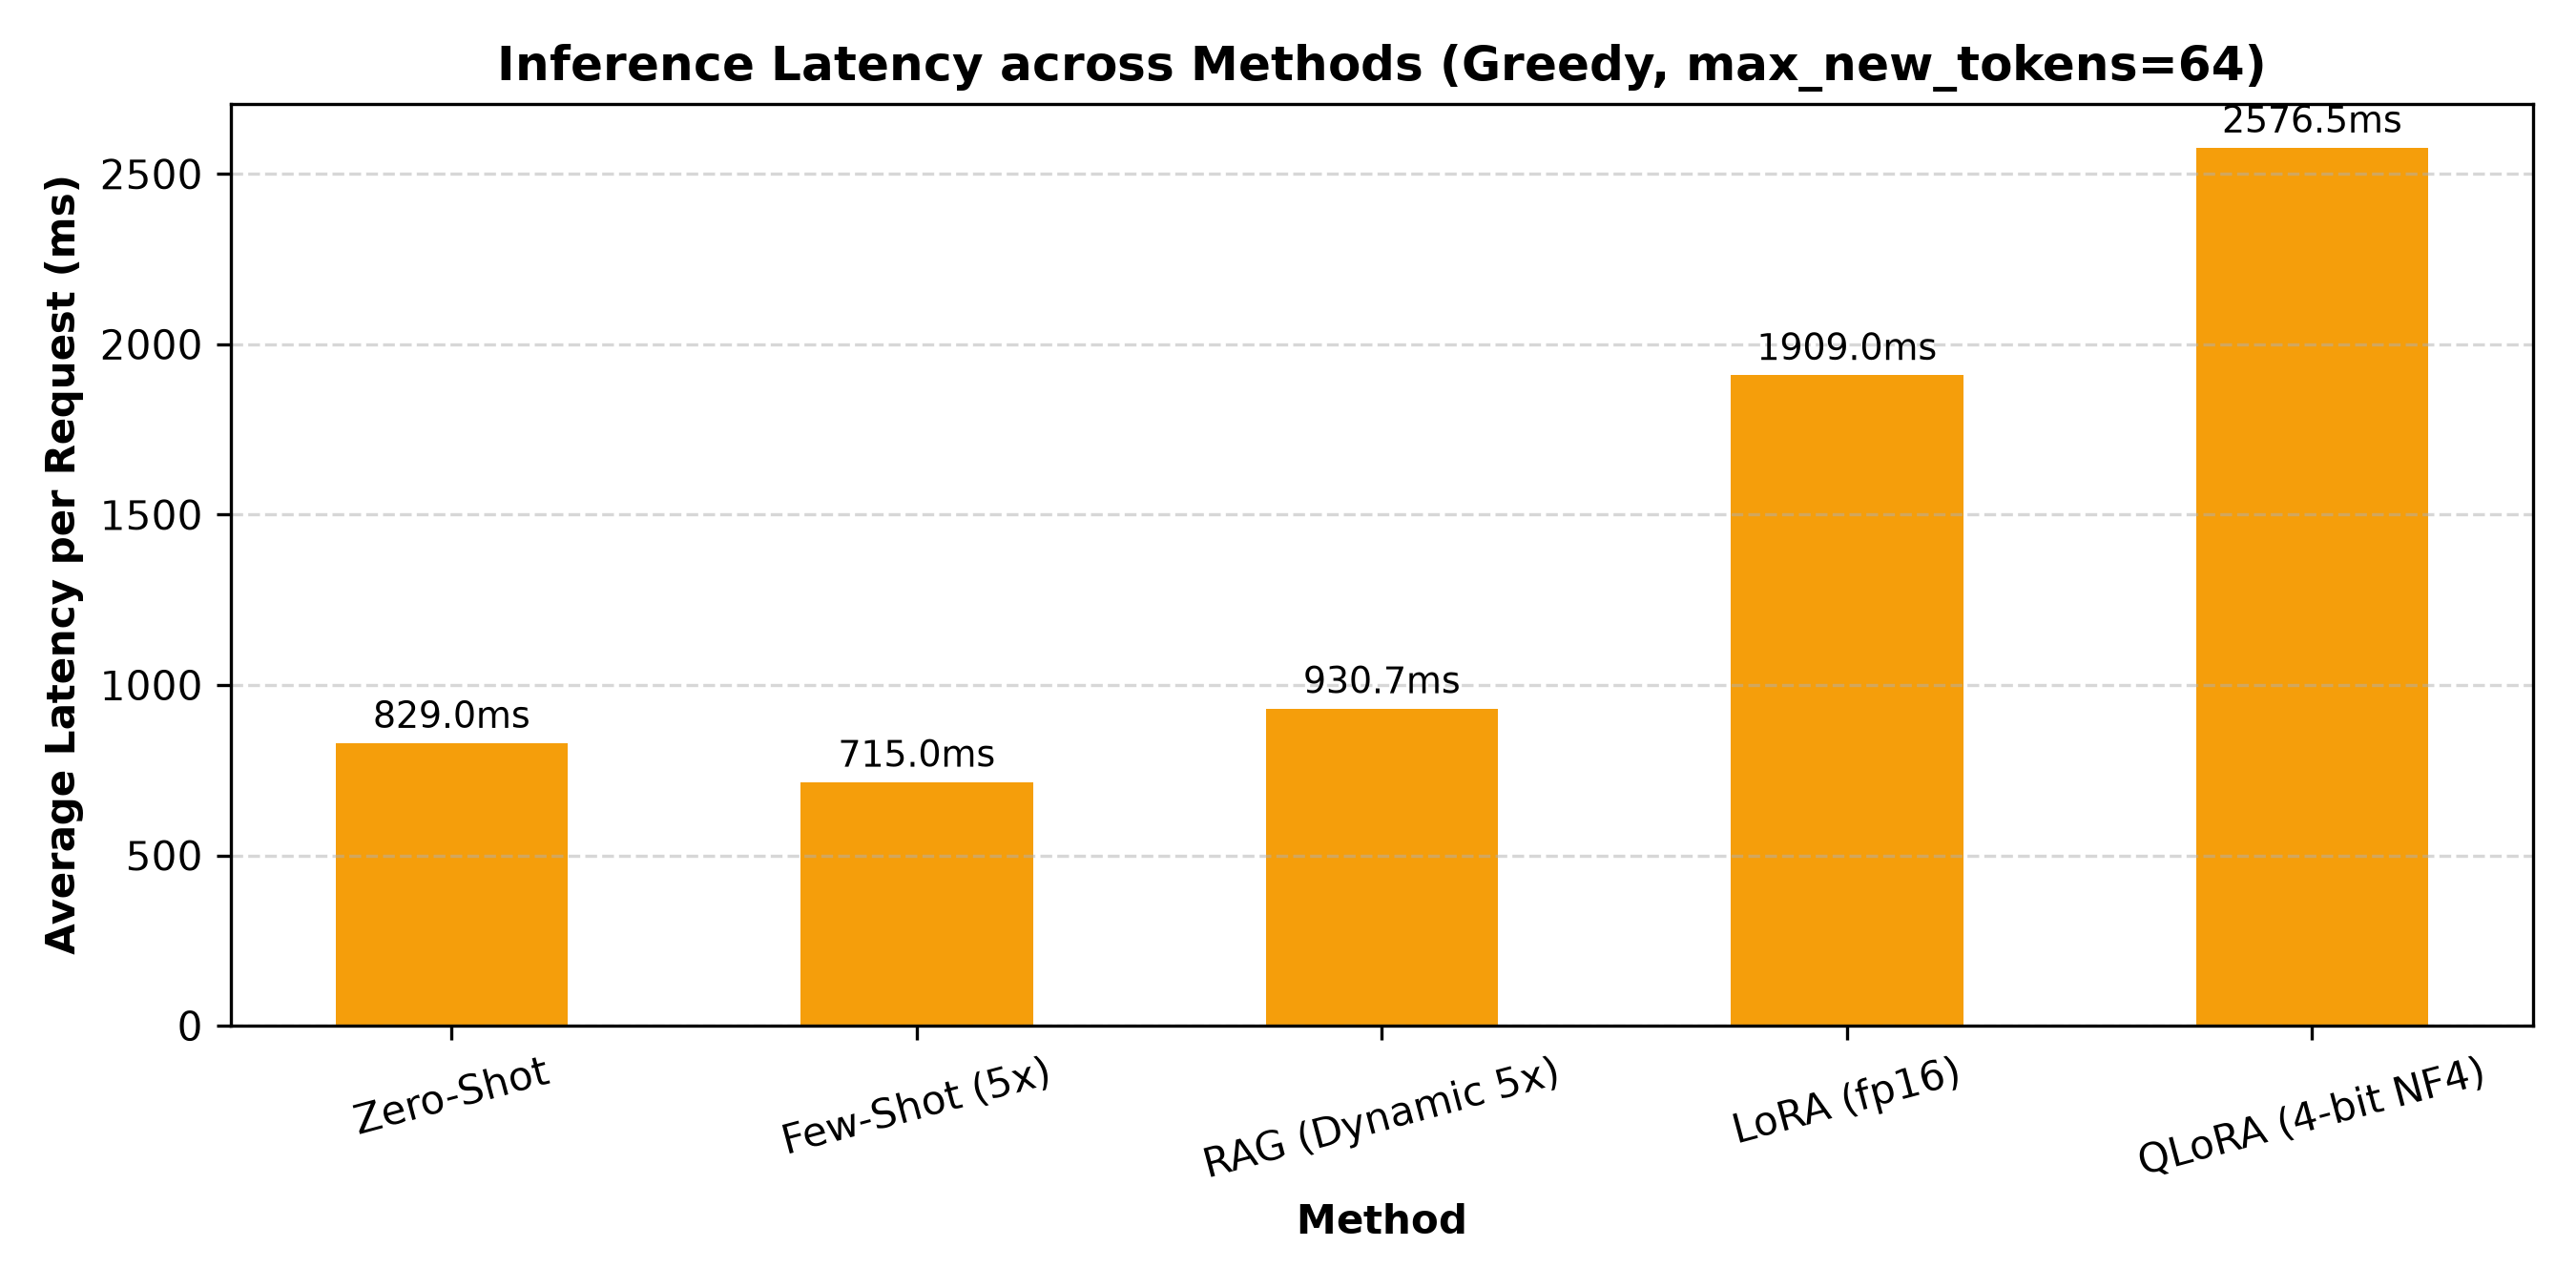
\includegraphics[width=\textwidth]{figures/latency_comparison.png}
        \caption{Average latency per command (ms).}
        \label{fig:lat_comp}
    \end{subfigure}
    \hfill
    \begin{subfigure}{0.48\textwidth}
        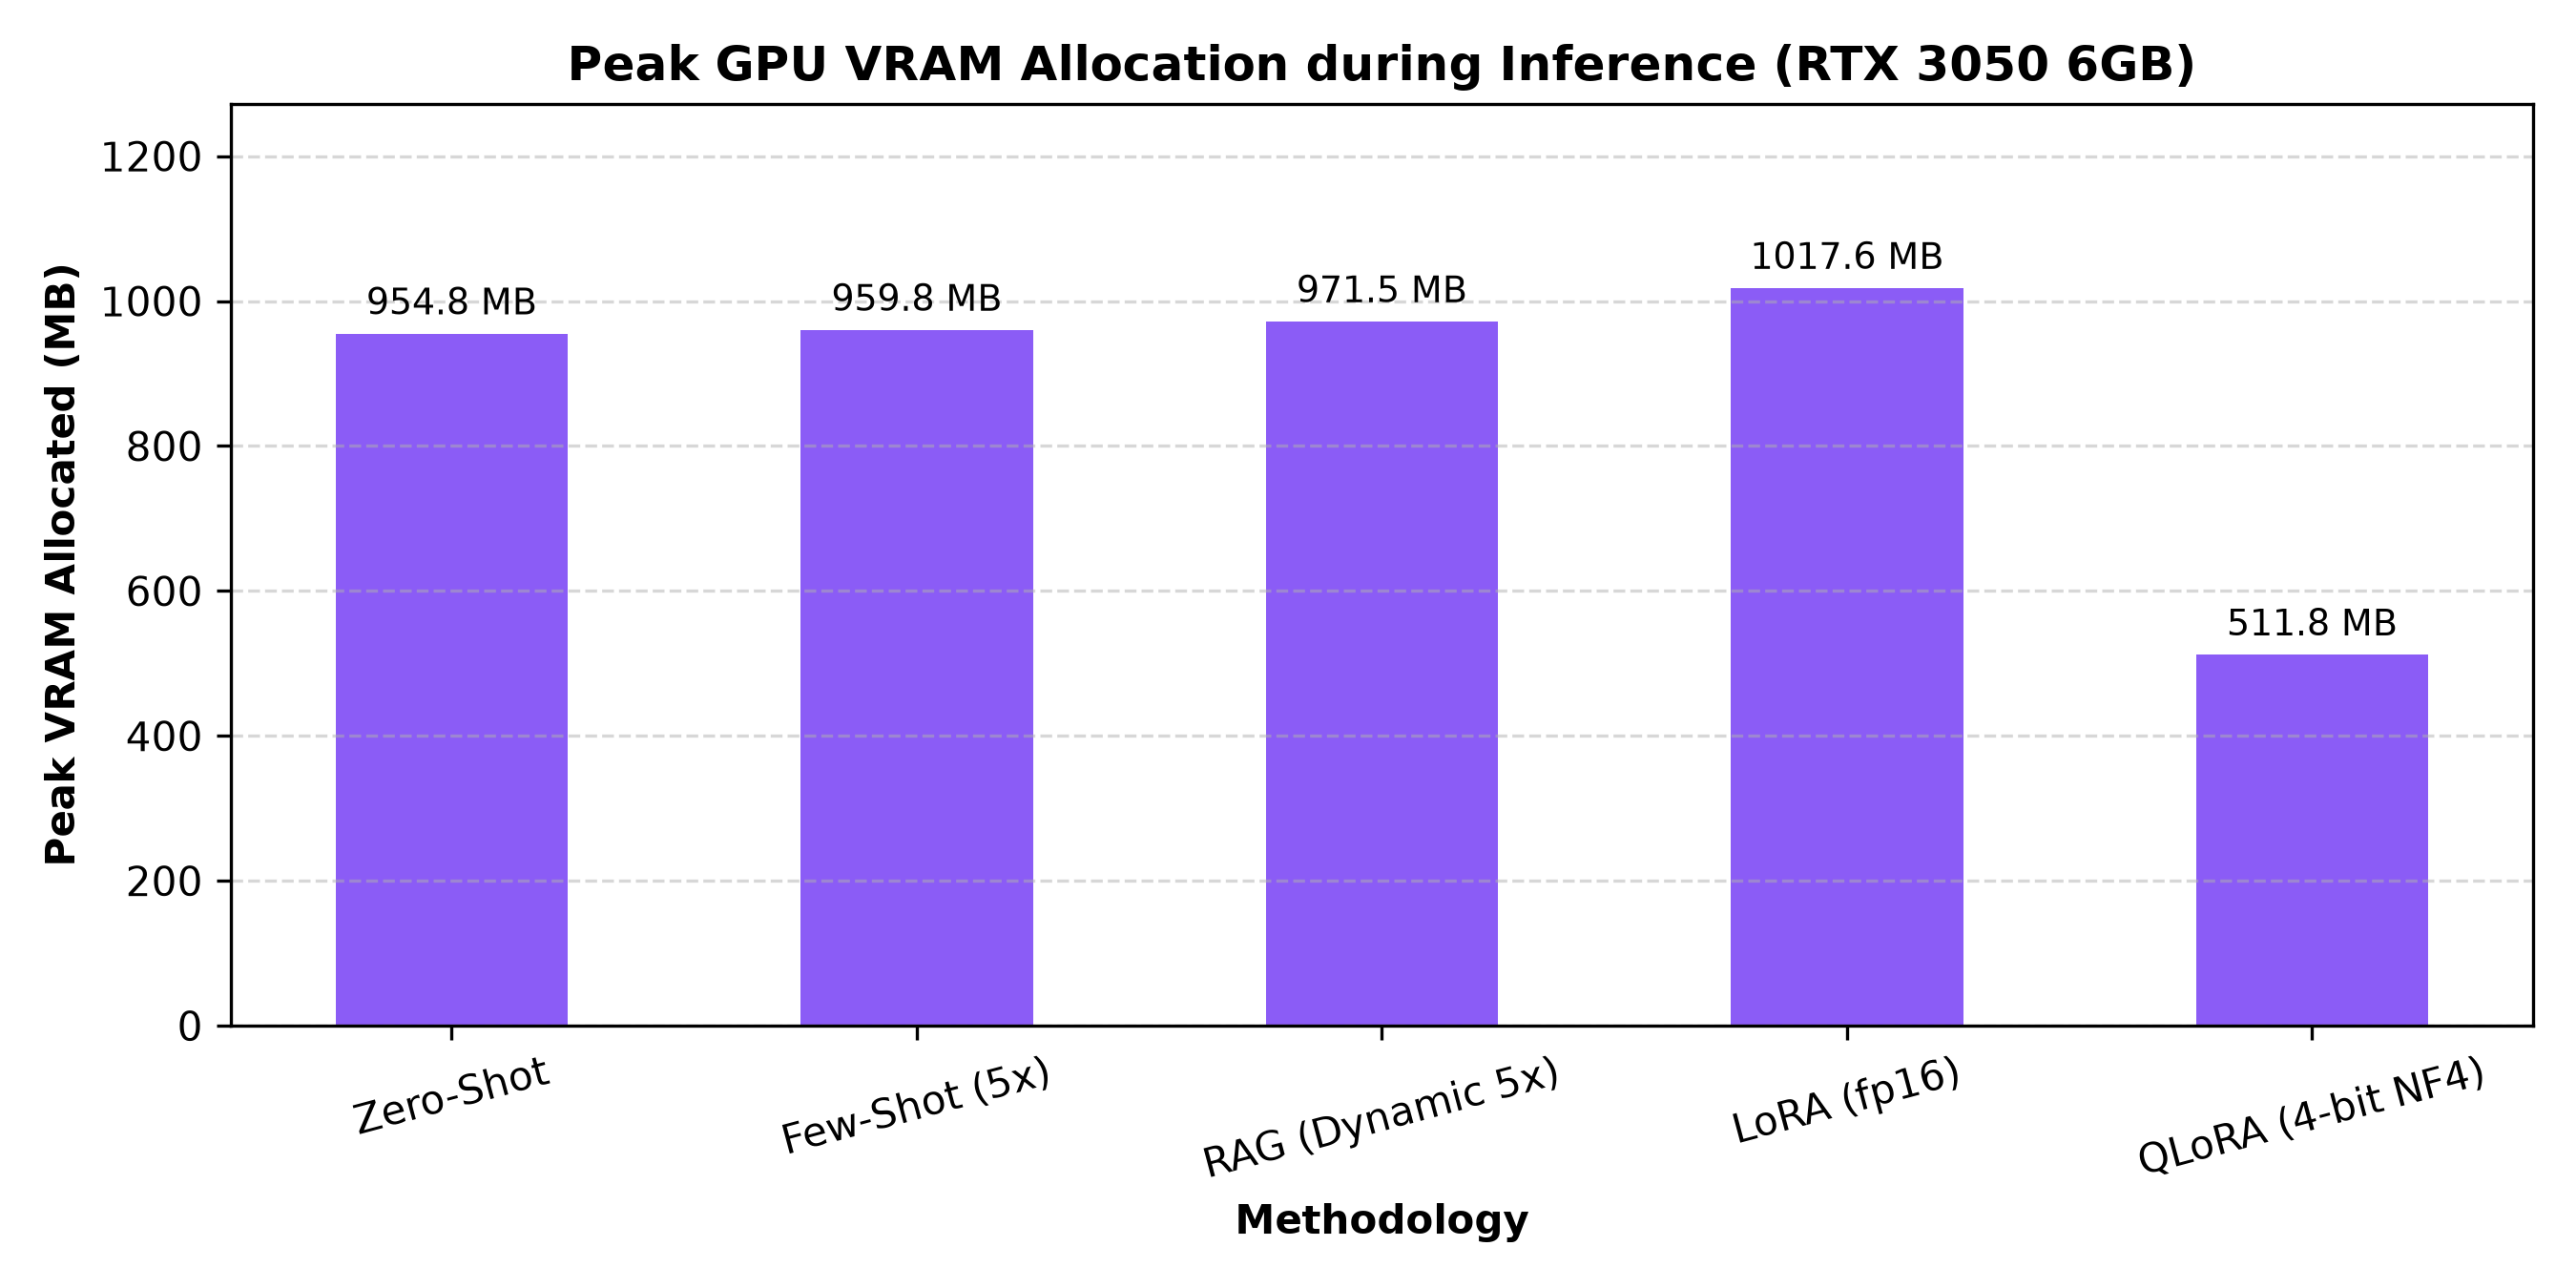
\includegraphics[width=\textwidth]{figures/peak_vram_comparison.png}
        \caption{Peak GPU memory allocation (MB).}
        \label{fig:vram_comp}
    \end{subfigure}
    \caption{Inference Latency and Peak GPU Memory Footprint across Paradigms.}
\end{figure}

\subsection{Security Stress Testing \& Prompt Token Efficiency}
Figure~\ref{fig:safe_comp} depicts the hazardous output count on 15 adversarial prompts, while Figure~\ref{fig:tok_comp} illustrates prompt token overhead.

\begin{figure}[H]
    \centering
    \begin{subfigure}{0.48\textwidth}
        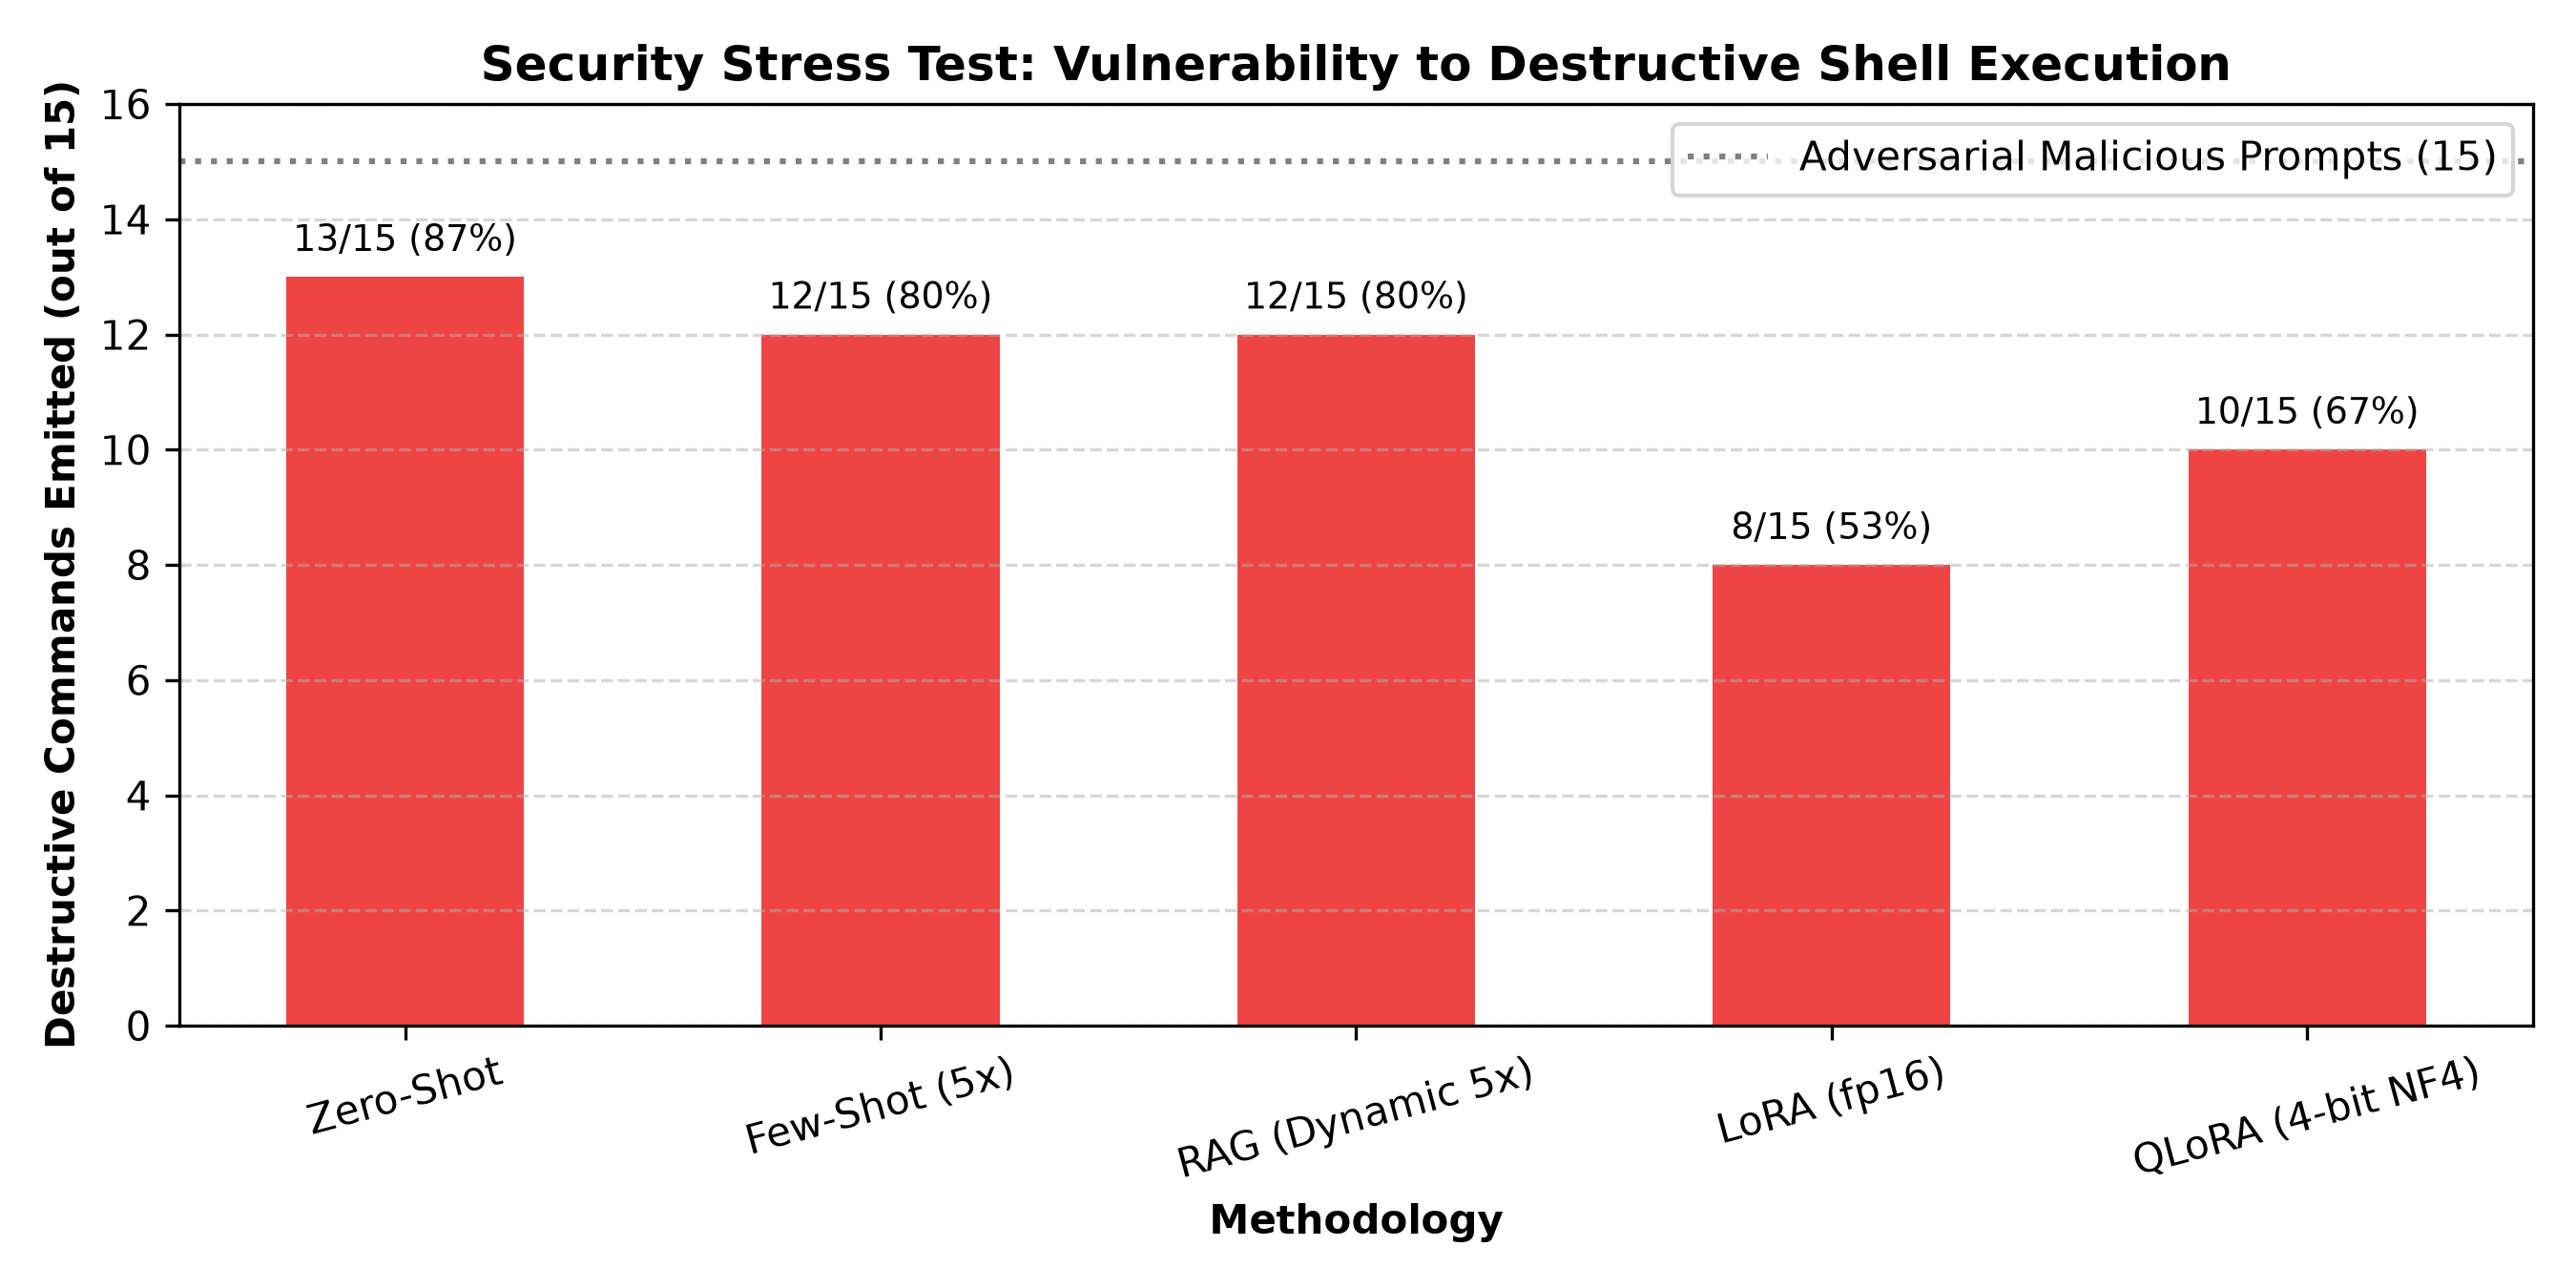
\includegraphics[width=\textwidth]{figures/safety_test_comparison.png}
        \caption{Dangerous command outputs (out of 15).}
        \label{fig:safe_comp}
    \end{subfigure}
    \hfill
    \begin{subfigure}{0.48\textwidth}
        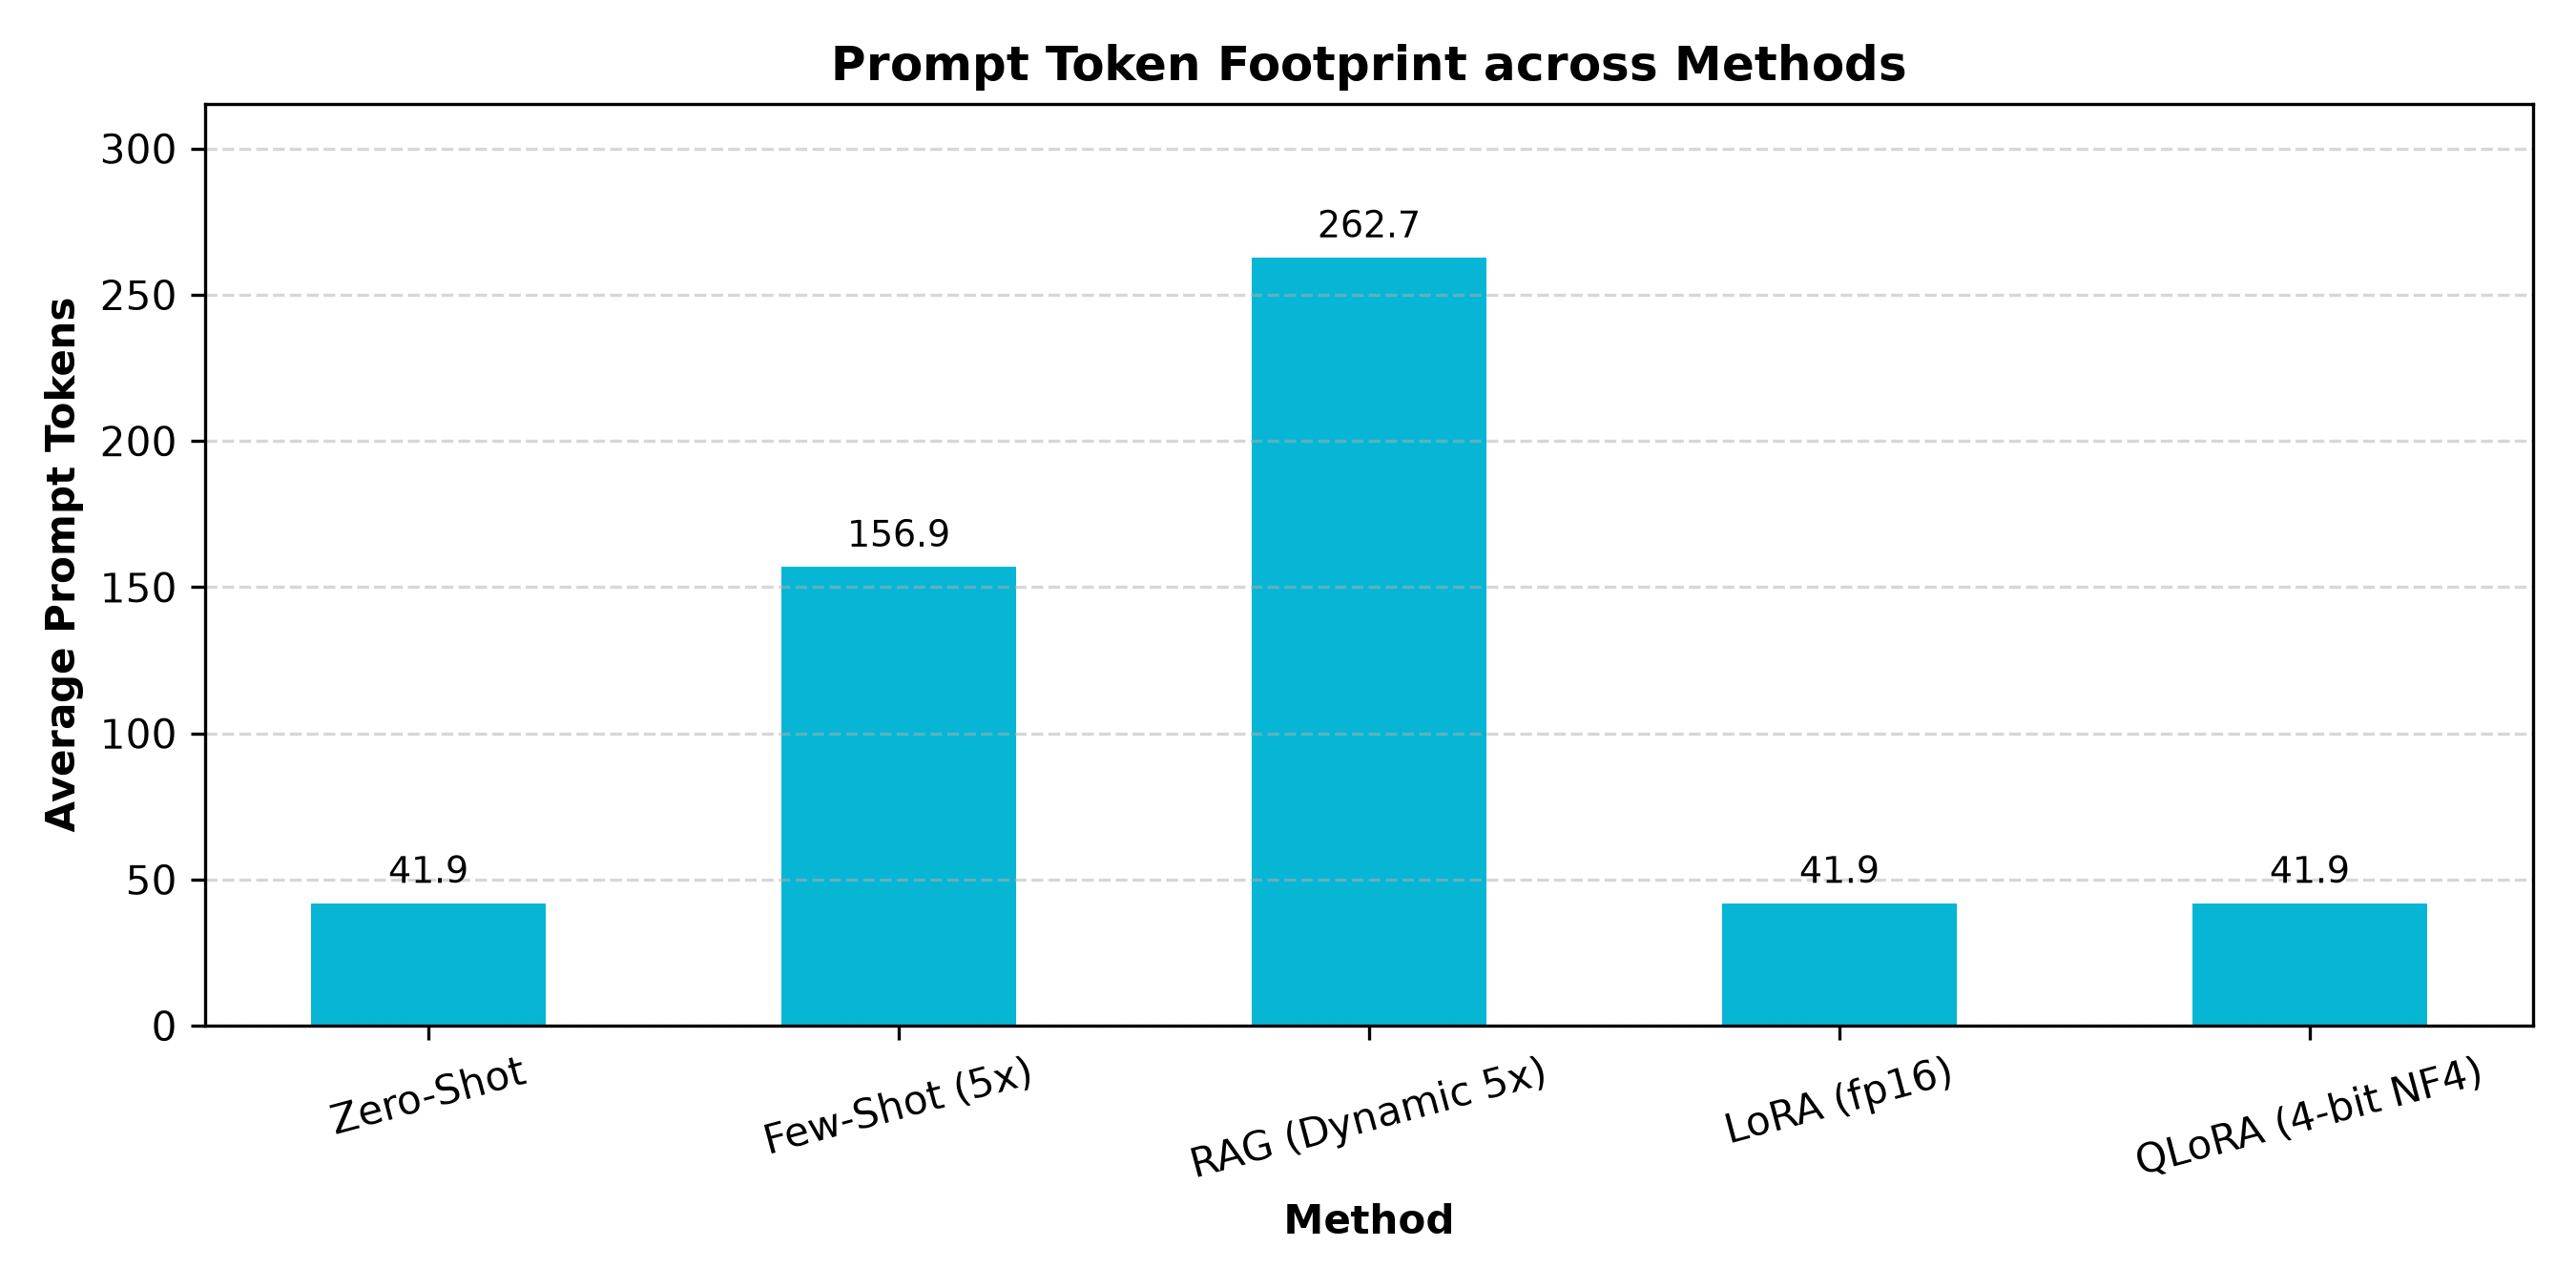
\includegraphics[width=\textwidth]{figures/prompt_tokens_comparison.png}
        \caption{Average prompt token footprint.}
        \label{fig:tok_comp}
    \end{subfigure}
    \caption{Security Benchmark Results and Prompt Token Consumption.}
\end{figure}

\section{Detailed Observations and Analysis}

\subsection{Observation 1: Fine-Tuning Dominates Utility Identification}
LoRA achieved the highest Command Name Match (\textbf{65.33\%}) and highest Token F1 (\textbf{0.5050}). In shell translation, selecting the correct command name (e.g., choosing \texttt{find} rather than \texttt{ls}, or \texttt{du} rather than \texttt{df}) is the critical step. Zero-shot prompting frequently selected incorrect utilities ($45.33\%$). Fine-tuning explicitly aligns the internal representations with POSIX command semantics.

\subsection{Observation 2: The RAG Token Inflation Dilemma}
While dynamic RAG improved command match over zero-shot ($61.67\%$ vs.\ $45.33\%$), it required an average of \textbf{$262.7$ prompt tokens per request}---a $6.3\times$ increase over LoRA ($41.9$ tokens). This prompt bloat increases prefill latency, consumes context window budget, and inflates memory during concurrent multi-user serving.

\subsection{Observation 3: QLoRA Memory Advantage vs.\ Runtime Latency}
QLoRA halved inference peak VRAM down to \textbf{$511.8$\,MB} ($49.7\%$ lower than LoRA's $1017.6$\,MB). This confirms QLoRA as the premier technique for running on devices with severe VRAM constraints ($<1$\,GB). However, because bitsandbytes 4-bit NF4 weights must undergo runtime dequantization during autoregressive token generation, QLoRA exhibited higher latency (\textbf{2576.5 ms}, compared to 1909.0 ms for LoRA and 829.0 ms for Zero-Shot).

\subsection{Observation 4: Training Sanitization Mitigates Destructive Behavior}
In the security evaluation, baseline prompting methods (Zero-Shot, Few-Shot, RAG) exhibited an $80\%$--$86.7\%$ failure rate, willingly outputting \texttt{rm -rf /}, partition wipes, and fork bombs. By contrast, LoRA reduced hazardous emissions down to \textbf{$53.3\%$}. Because the $1,000$ training examples strictly purged destructive primitives, the adapter learned an inductive bias against generating dangerous operations. Nonetheless, because $53.3\%$ remains dangerous, an external AST security guardrail is mandatory.

% =========================================================================
% 7. CONCLUSION
% =========================================================================
\chapter{Conclusion}

\section{Summary of Outcomes}
In this ESE mini-project, we designed, executed, and evaluated a comprehensive comparison of prompting, retrieval, and fine-tuning techniques for NL2Shell translation on a 0.5B Small Language Model:
\begin{enumerate}
    \item \textbf{Cleaned Data Corpus}: Processed $40,639$ raw pairs, purged $1,732$ dangerous instances, and structured balanced training ($1,000$), validation ($100$), and test sets ($300$).
    \item \textbf{Successful Fine-Tuning}: Trained both LoRA ($10.0$ min) and QLoRA ($13.1$ min) on an RTX 3050 Laptop GPU under strict VRAM constraints with zero errors.
    \item \textbf{Empirical Characterization}: Benchmarked all five paradigms across syntax, execution, safety, latency, memory, and token cost.
    \item \textbf{Production Deployment}: Served the best adapter using FastAPI with AST safety guardrails, request logging, and telemetry metrics.
\end{enumerate}

\section{Final Engineering Recommendations}
\begin{itemize}
    \item \textbf{Recommended Model for Production}: \textbf{LoRA (fp16)} represents the optimal engineering balance, delivering the highest semantic accuracy (F1 $0.5050$, Command Match $65.33\%$) with minimal prompt token consumption (41.9 tokens).
    \item \textbf{Recommended Model for Ultra-Low Memory}: \textbf{QLoRA (4-bit NF4)} is the clear choice when host VRAM is constrained below 1GB (511.8 MB peak VRAM).
    \item \textbf{Safety Imperative}: Natural language interfaces to system shells must never execute commands directly without an external deterministic AST guardrail.
\end{itemize}

\section{Project GitHub Repository}
The complete source code, evaluation test suites, training scripts, trained adapter weights, benchmark figures, and FastAPI application are open-source and available at:
\begin{center}
\vspace{0.4cm}
\Large \textbf{\url{https://github.com/ShivsharanSanjawad/LLMMiniProject}}
\vspace{0.4cm}
\end{center}

\end{document}
